%%% LaTeX Template: Article/Thesis/etc. with colored headings and special fonts
%%%
%%% Source: http://www.howtotex.com/
%%% Feel free to distribute this template, but please keep to referal to http://www.howtotex.com/ here.
%%% February 2011
%%%
%%% Modified May 2018 by CDM

%%%  Preamble
\documentclass[11pt,letterpaper]{article}
\usepackage[margin=1.0in]{geometry}
\usepackage[T1]{fontenc}
\usepackage[bitstream-charter]{mathdesign}
\usepackage[latin1]{inputenc}					
\usepackage{amsmath}						
\usepackage{xcolor}
\usepackage{cite}
\usepackage{hyphenat}
\usepackage{graphicx}
\usepackage{float}
\usepackage{subfigure}
\usepackage{sectsty}
\usepackage[compact]{titlesec} 
\usepackage[tablegrid]{vhistory}
\allsectionsfont{\color{accentcolor}\scshape\selectfont}

%%% Definitions
\definecolor{accentcolor}{rgb}{0.0,0.0,0.5} 
\newcommand{\teamname}{Team Name}
\newcommand{\productname}{Product Name}
\newcommand{\coursename}{CSE 4316: Senior Design I}
\newcommand{\semester}{Spring 2018}
\newcommand{\docname}{System Requirements Specification}
\newcommand{\department}{Department of Computer Science \& Engineering}
\newcommand{\university}{The University of Texas at Arlington}
\newcommand{\authors}{Alan Turing \\ Grace Hopper \\ John Von Neumann \\ Ada Lovelace \\ Charles Babbage}

%%% Headers and footers
\usepackage{fancyhdr}
	\pagestyle{fancy}						% Enabling the custom headers/footers
\usepackage{lastpage}	
	% Header (empty)
	\lhead{}
	\chead{}
	\rhead{}
	% Footer
	\lfoot{\footnotesize \teamname \ - \semester}
	\cfoot{}
	\rfoot{\footnotesize page \thepage\ of \pageref{LastPage}}	% "Page 1 of 2"
	\renewcommand{\headrulewidth}{0.0pt}
	\renewcommand{\footrulewidth}{0.4pt}

%%% Change the abstract environment
\usepackage[runin]{abstract}			% runin option for a run-in title
%\setlength\absleftindent{30pt}			% left margin
%\setlength\absrightindent{30pt}		% right margin
\abslabeldelim{\quad}	
\setlength{\abstitleskip}{-10pt}
\renewcommand{\abstractname}{}
\renewcommand{\abstracttextfont}{\color{accentcolor} \small \slshape}	% slanted text

%%% Start of the document
\begin{document}

%%% Cover sheet
{\centering \huge \color{accentcolor} \sc \textbf{\department \\ \university} \par}
\vspace{1 in}
{\centering \huge \color{accentcolor} \sc \textbf{\docname \\ \coursename \\ \semester} \par}
\vspace{0.5 in}
\begin{figure}[h!]
	\centering
   	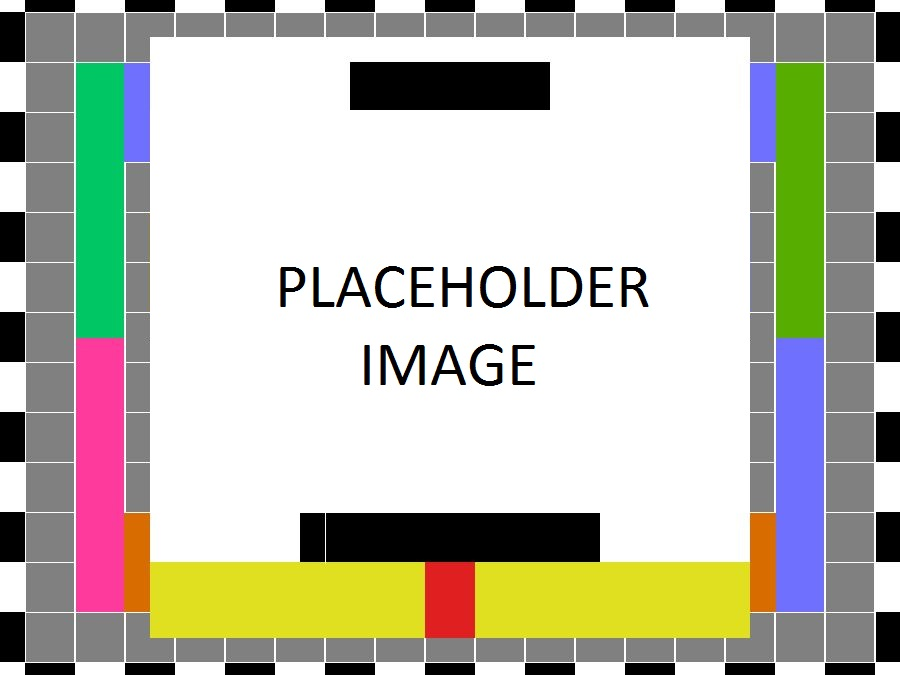
\includegraphics[width=0.60\textwidth]{images/test_image}
\end{figure}
\vspace{0.5 in}
{\centering \huge \color{accentcolor} \sc \textbf{\teamname \\ \productname} \par}
\vspace{0.5 in}
{\centering \large \sc \textbf{\authors} \par}
\newpage


%\vspace{1 in}
%\centerline{January 13th, 2012}
%\newpage

%%% Revision History
\begin{versionhistory}
  	\vhEntry{0.1}{10.01.2015}{GH}{sandesh donnnnn}
  	\vhEntry{0.2}{10.05.2015}{AT|GH}{tara bhain}
  	\vhEntry{0.3}{10.12.2015}{AT|GH}{stmpo line}
  	\vhEntry{1.0}{10.20.2015}{AT|GH|CB}{official release}
  	\vhEntry{1.1}{10.31.2015}{AL}{added customer change requests}
\end{versionhistory}
\newpage

%%% Table of contents
\setcounter{tocdepth}{3}
\tableofcontents
\newpage

%%% List of figures and tables (optional)
\listoffigures
%\listoftables
\newpage

\section{Product Concept}
We humans are surrounded by lots of items. Those items might be very important or might not be important at all. With having to interact with lots of items it is pretty hard for us to remember what items are needed and where it is located.\\
Pocket-self is the inventory tracking app that helps people to store and record the items that are important in a organized manner. With the help of the app users will be able to record the items in the database and later on retrieve it when needed. Users will be able to choose the particular self or the location that he/she wants to store the item. Then the app helps to enter the location and the item and saves the information in the database. Users will also be able to scan the item rather than having to enter the information manually. So, when the user needs the specific item then he can just search the app and it will tell where exactly is the item located.


\subsection{Purpose and Use}
The purpose of the app is to make the life of user easier by organizing all the items as inventory in an organized fashion. The main goal of app is to store the information of the app in database and retrieve quickly when needed. When the user defines the location of the storage and provides the information about the item that they want to store, then the user can retrieve the information in the future just by doing the quick search. The app will also provide notification about the expiry date and vital information about the product in timely manner. Basically the app is used for storing items information and retrieve the location and information quickly when needed.

\subsection{Intended Audience}
This app is specifically intended for the people who want to organize the items that they have in their houses but, it can also be used for business to record the inventory if needed. This app is more useful for collectors. As for the collectors they have numerous amount of same type of the item. For example, the user might have collection of beverages or books. So, what he can do is he can enter the information and the location of where all the items he wants to store. Then, in future he can retrieve the item with ease.


\begin{figure}[hbt!]
	\centering
   	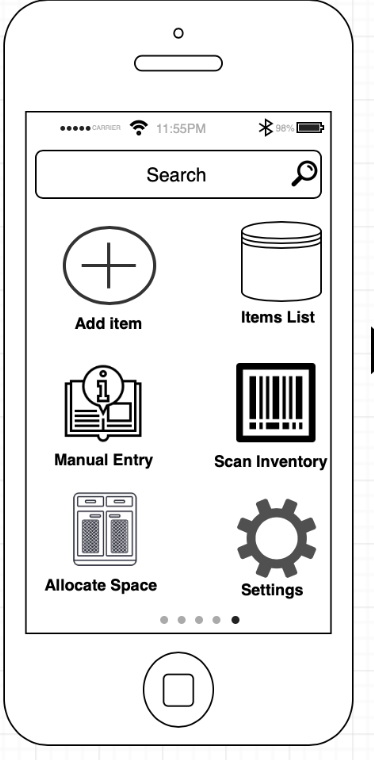
\includegraphics[width=0.60\textwidth]{images/product.PNG}
    \caption{Basic UI of the application}
\end{figure}

\newpage
\section{Product Description}
PocketShelf is an IOS/ Android based mobile application which allow user to keep their items in available space, which is previously created by user. We called it "PocketShelf" because, basically one is carrying all the shelf inside his/her pocket, like s/he can find his/her item just in a click. Not only that s/he can add an item in the app and app will decide where to keep that item, and it will ask some image of that item after which they can put that item on the given shelf and can forget where they kept it. All the remembering things will be done by the app, on top of it, our app will allow user to see the actual image of that item, so that the user can know that the item s/he is looking for is the exact item on the shelf before they grab it which will save their time and effort. Based on the items that can be added to the app, our application have different versions. 


\subsection{Features \& Functions}
"PocketShelf" is an inventory app, that can keep track of any item that user wants. We used Augmented reality as our key feature of the application. Where user can see the item before s/he approach to grab it. Which might be helpful in the sense that it will save the user effort and time spent, it s/he known that they are getting the right thing. Our app not only keep track of the item but able to sort the items based on the expiration dates and can notify the user if the item is expiring soon. Time frame to notify user can be pre- defined by the user at the time of its entry. Our app use the online database to save every entry by the user and had to be encrypted before it goes to the database, all the data had to flow through the server. So, user have to be online to be able to use the app. We had PIN protection as an extra feature on the app, where if the user want not to show the item location to other user using the same app on same device. Which we found cool feature if the user wants to secure his/her valuable items somewhere in the shelf.


\subsection{External Inputs \& Outputs}
 Initial version of PocketShelf is vary basic version of inventory app, which is fully based on the user input rather then machine learning's predictions. Each and every input should go through user.User can scan the bar code of the item to be stored(optional), user have to give unique name to the item to be store, user can add some notes about the item in item description field, user must dive the quantity of item to be stored in the shelf, it can be one or more. If the item have expiration date and user want to keep track of the expiration of any item on the shelf, during entry they can specify the expiration date and enable the notification before the specified date. If user does not want other user to see the location of the item, s/he can enable PIN protection for the location. User must add the picture of the item to be stored before adding to the database. Once user provide all valid input, user can press add button after which app will give the available location with a QR-code, user can save the QR-code for his record. Later if the user wants to retrieve some item, s/he can scan the QR, where the app will show the picture of the item up on the QR, to help user to able to identify the item. Once user pick the item S/he should input quantity picked from the location. If the location is PIN protected, during QR scan app will ask PIN to verify the user before reveling the item picture and item location. 
\pagebreak

\subsection{Product Interfaces}
These are some of the user interface. Where Home screen is shown as soon as application is launched, if user wants to add item app will launch adding item screen and so on. We had implemented our interface in such a way that even a color blind person can easily use our app.
\\Home Screen
\begin{figure}[hbt!]
                	\centering
                   	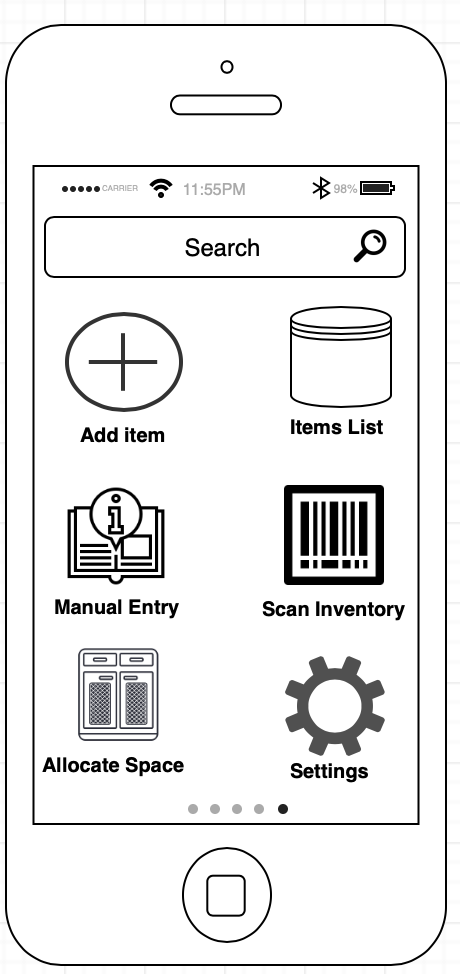
\includegraphics[width=0.19\textwidth]{images/home}
                    \caption{Home Screen}
                \end{figure}

Adding Item.
\begin{figure}[hbt!]
                	\centering
                   	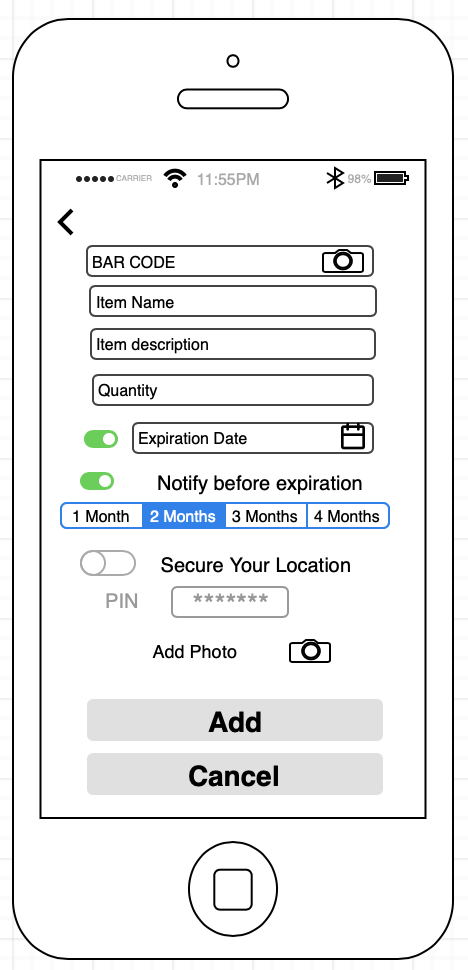
\includegraphics[width=0.19\textwidth]{images/adding}
                    \caption{Adding item}
                \end{figure}
                
\pagebreak
Product Search.
\begin{figure}[hbt!]
                	\centering
                   	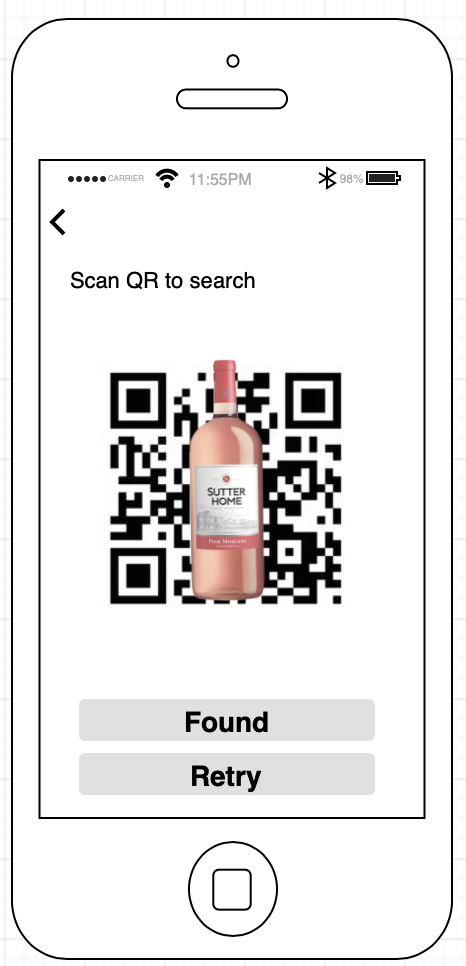
\includegraphics[width=0.19\textwidth]{images/search}
                    \caption{Product search using QR}
                \end{figure}
\\Product Found.
\begin{figure}[hbt!]
                	\centering
                   	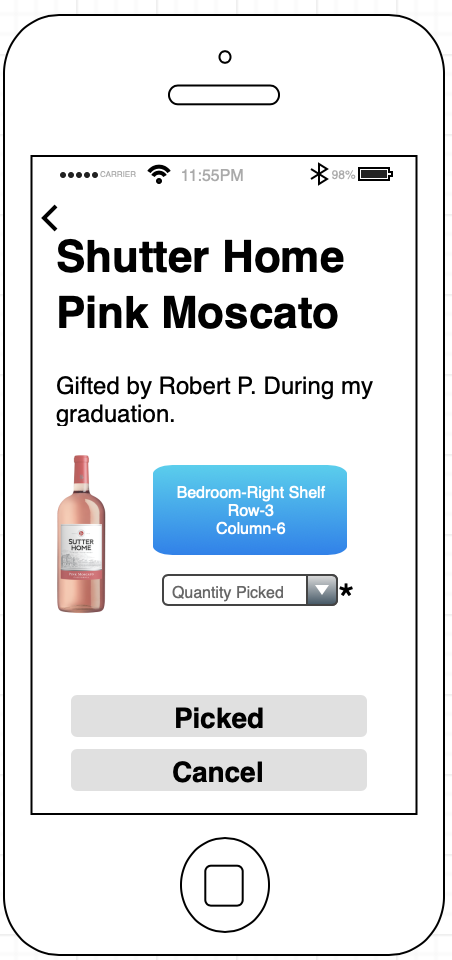
\includegraphics[width=0.19\textwidth]{images/pick}
                    \caption{Picking product once found}
                \end{figure}
\pagebreak
\\Adding New Shelf.
\begin{figure}[hbt!]
                	\centering
                   	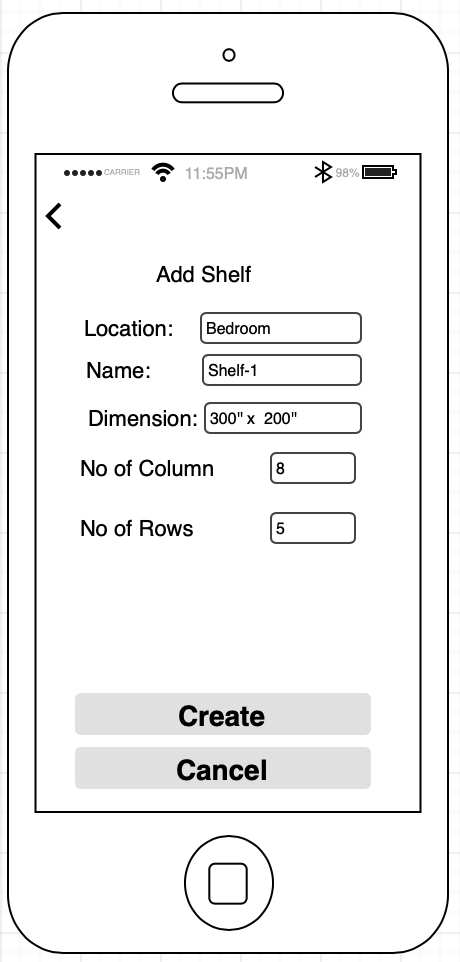
\includegraphics[width=0.19\textwidth]{images/shelf}
                    \caption{Adding Shelf}
                \end{figure}

\newpage
\section{Customer Requirements}
The system aims at providing these features and functions in the app as per the requirements gathered from different sources. With the help of these core defined functionality users will be able to manage and store their inventory in easily reachable and secure manner. The main Customer Requierment for are app are:

\subsection{Registration}
\subsubsection{Description}
Application shall allow the first time user to register a account.
\begin{itemize}
\item User should provide valid Email
\item User should provide unique username
\item User should provide at least 6 alpha numeric password.
\item User should provide three security questions.
\item User should provide the account type(individual/business).
\end{itemize}

\subsubsection{Source}
CSE Senior Design Project Specification.
\subsubsection{Constraints}
\begin{itemize}
\item User must have a valid email. 
\end{itemize}

\subsubsection{Standards}
All the user information must be in encryption using \textit{MD5 encryption}.
\subsubsection{Priority}

\begin{itemize}
\item Critical\\ \\
\end{itemize}

\subsection{Login}
\subsubsection{Description}
Application shall allow the registered user to login their account with registered username and its password. In the login page application shall allow user some way to reset their password if forgotten. 
\subsubsection{Source}
CSE Senior Design Project Specification.
\subsubsection{Constraints}
\begin{itemize}
\item User must be registered. 
\end{itemize}
\subsubsection{Standards}
All the input must be verified before using it to any queries to prevent SQL injection. 
\subsubsection{Priority}
\begin{itemize}
\item Critical\\ \\
\end{itemize}

\subsection{Allocation of space}
\subsubsection{Description}
Application shall allow the valid user to create customized shelf, based on the types of shelf s/he have, in order to store the items. For which:
\begin{itemize}
\item User should provide Name of the shelf
\item User should provide the location for the shelf
\item User should provide the numbers of rows and column in the shelf.
\end{itemize}
\subsubsection{Source}
Customer
\subsubsection{Constraints}
\begin{itemize}
\item Should be logged in to an account.
\end{itemize}
\subsubsection{Standards}
N/A
\subsubsection{Priority}
\begin{itemize}
\item Moderate \\ \\
\end{itemize}

\subsection{Adding item to Inventory}
\subsubsection{Description}
Application shall allow User to add item to their existing shelf.
\begin{itemize}
\item User must provide Item Name.
\item user must provide Item Description.
 If item is Beverage
\begin{itemize}
\item User may provide the name of Brewery.
\item User may provide Style of Beverage.
\item User may specify the format of the container.
\end{itemize}
\item User Can provide the expiration date of the item if any.
\item User must provide the quantity they want to store.
\item User can select an option to be notified before the expiration of any item in the shelf.
\item User can set up a pin to secure the position of the specific item for not letting other user to know its position if searched.
\end{itemize}

\subsubsection{Source}
Chris Conly
\subsubsection{Constraints}
\begin{itemize}
\item User Should have at least one empty position on the shelf.
\end{itemize}
\subsubsection{Standards}
\begin{itemize}
\item System should generate some form of notification for successfully adding  
\item System should generate some thing to be able to locate same item in future.
\end{itemize}
\subsubsection{Priority}
\begin{itemize}
\item Highly.\\ \\
\end{itemize}

\subsection{Modify Specification}
\subsubsection{Description}
System shall allow the authorized user to modify any thing from the added item. 
\begin{itemize}
\item User can change the Item name or quantity added of so other description of the item even after it is added to the shelf.
\end{itemize}
\subsubsection{Source}
Team member(Utsav Acharya).
\subsubsection{Constraints}
\begin{itemize}
\item Should be authorized user for that item.
\item Item should be in the shelf.
\end{itemize}
\subsubsection{Standards}
N/A
\subsubsection{Priority}
\begin{itemize}
\item LOW.\\ \\
\end{itemize}

\subsection{Search Using QR}
\subsubsection{Description}
System shall generate unique QR for every entered item and users shall be able to search for the item using specific QR code.
\subsubsection{Source}
CSE Senior Design Project Specification
\subsubsection{Constraints}
\begin{itemize}
\item User must be a valid registered user.
\item User must have working camera in their mobile phone to scan the QR.
\item User must have the valid unhampered QR code. 
\end{itemize}
\subsubsection{Standards}
N/A
\subsubsection{Priority}
\begin{itemize}
\item HIGH.\\ \\
\end{itemize}

\subsection{Manual Search}
\subsubsection{Description}
Users shall be allowed to search the item just by using product name.
\begin{itemize}
\item User can just type the name of the item in the search bar to view result about their query.
\item The search bar will provide the live search feature.
\end{itemize}
\subsubsection{Source}
Cse Senior Design Project Specification 
\subsubsection{Constraints}
\begin{itemize}
\item User must be a valid registered user.
\item User must have a working keyboard to provide input.
\end{itemize}
\subsubsection{Standards}
N/A
\subsubsection{Priority}
\begin{itemize}
\item Critical.\\ \\
\end{itemize}

\subsection{Private Inventory}
\subsubsection{Description}
Users shall be able to keep the location of the item to private  by providing pin to lock location of certain item. 
\begin{itemize}
\item User should provide pin to make the items location private.
\item User should provide pin after searching to reveal the location of inventory.
\end{itemize}
\subsubsection{Source}
Team member(Sudip Kandel).
\subsubsection{Constraints}
\begin{itemize}
\item Must have a valid working keyboard.
\item Must be a valid registered member.
\end{itemize}
\subsubsection{Standards}
\begin{itemize}
    \item Pin number must have four digits.
\end{itemize}
\subsubsection{Priority}
\begin{itemize}
\item Low.\\ \\
\end{itemize}

\subsection{Display result in Augmented Reality}
\subsubsection{Description}
System shall display the result to the user in Augmented reality.
\begin{itemize}
\item User will be able to view the picture of the exact item in the Augmented reality.
\end{itemize}
\subsubsection{Source}
Team member(Sudip Kandel).
\subsubsection{Constraints}
\begin{itemize}
\item Item must be already entered in the inventory.
\item User must be a valid registered user.
\item User must have a working camera.
\end{itemize}
\subsubsection{Standards}
\begin{itemize}
    \item Size of the AR must not be bigger than the size of actual item.
\end{itemize}
\subsubsection{Priority}
\begin{itemize}
\item LOW.\\ \\
\end{itemize}
\newpage
\section{Packaging Requirements}
Since our product is an mobile application. It is not required to pack physically. When finished our product will be delivered as a mobile application. Our app will be uploaded on the ios and android application store and the customers will be able to download the app.

\subsection{Requirement Name}
\subsubsection{Description}
Our PocketShelf App can be downloaded by the customers from app stores. It will work for both android and ios.
\subsubsection{Source}
Source
\subsubsection{Constraints}
android and ios version ?
\subsubsection{Standards}
wifi network
\subsubsection{Priority}
Critical
\newpage
\section{Performance Requirements}
The performance of the app has significance important to make a beverage inventory fast, easy and accurate. Since the inventory app is finding the beverage products from shelves or suggesting the space in the shelves  after scanning the QR Code, if performance is not good the app will mess up inventory list of beverage product, customers will not use it for inventory of beverage products. Inventory operation should perform fast and accurate. App will not drain the battery of the device and lasts as long as the battery of the mobile lasts and setup is not difficult, customers just have to install the application on their smart phones.

\subsection{The application should start within  1 to 2 seconds.}
\subsubsection{Description}
Customer can open the application as fast as possible and able to make inventory manually, scanning bar-code or QR code. The application should be ready to inventory.
\subsubsection{Source}
The Nepster
\subsubsection{Constraints}
The application should open, scan bar-code or QR code very fast.
\subsubsection{Priority}
High
\subsection{The application should retrieve the data very fast and accurate.}
\subsubsection{Description}
System should retrieve the inventory data of beverage product accurate and fast as much as possible. Database should keep records of every update of the inventory.
\subsubsection{Source}
The Nepster
\subsubsection{Constraints}
Application should connected with wifi or internet. The application should retrieve inventory data accurate and update every records of inventory.The platform should be IOs and Android 
\subsubsection{Priority}
High
\subsection{The application support the workload.}
\subsubsection{Description}
System should support free up to 5000 items and needs premium account for more than 5000 items.
\subsubsection{Source}
The Nepster
\subsubsection{Constraints}
Application should connected with wifi or internet and able to handle up to 1 millions users without any performance issues.The platform should be IOs and Android.
\subsubsection{Priority}
High
\newpage
\section{Safety Requirements}
Include a header paragraph specific to your product here. Safety requirements might address items specific to your product such as: no exposure to toxic chemicals; lack of sharp edges that could harm a user; no breakable glass in the enclosure; no direct eye exposure to infrared/laser beams; packaging/grounding of electrical connections to avoid shock; etc.

\subsection{Laboratory equipment lockout/tagout (LOTO) procedures}
\subsubsection{Description}
Any fabrication equipment provided used in the development of the project shall be used in accordance with OSHA standard LOTO procedures. Locks and tags are installed on all equipment items that present use hazards, and ONLY the course instructor or designated teaching assistants may remove a lock. All locks will be immediately replaced once the equipment is no longer in use.
\subsubsection{Source}
CSE Senior Design laboratory policy
\subsubsection{Constraints}
Equipment usage, due to lock removal policies, will be limited to availability of the course instructor and designed teaching assistants.
\subsubsection{Standards}
Occupational Safety and Health Standards 1910.147 - The control of hazardous energy (lockout/tagout).
\subsubsection{Priority}
Critical

\subsection{National Electric Code (NEC) wiring compliance}
\subsubsection{Description}
Any electrical wiring must be completed in compliance with all requirements specified in the National Electric Code. This includes wire runs, insulation, grounding, enclosures, over-current protection, and all other specifications.
\subsubsection{Source}
CSE Senior Design laboratory policy
\subsubsection{Constraints}
High voltage power sources, as defined in NFPA 70, will be avoided as much as possible in order to minimize potential hazards.
\subsubsection{Standards}
NFPA 70
\subsubsection{Priority}
Critical

\subsection{RIA robotic manipulator safety standards}
\subsubsection{Description}
Robotic manipulators, if used, will either housed in a compliant lockout cell with all required safety interlocks, or certified as a "collaborative" unit from the manufacturer.
\subsubsection{Source}
CSE Senior Design laboratory policy
\subsubsection{Constraints}
Collaborative robotic manipulators will be preferred over non-collaborative units in order to minimize potential hazards. Sourcing and use of any required safety interlock mechanisms will be the responsibility of the engineering team.
\subsubsection{Standards}
ANSI/RIA R15.06-2012 American National Standard for Industrial Robots and Robot Systems, RIA TR15.606-2016 Collaborative Robots
\subsubsection{Priority}
Critical

\newpage
\section{Maintenance \& Support Requirements}


\subsection{Compatibility}
\subsubsection{Description}

-PocketShelf shall not crash, force close, freeze, or otherwise function abnormally on any targeted device.\\
-The app runs on the latest public version of the android and iOS.
\subsubsection{Source}
Customer
\subsubsection{Standards}
\begin{itemize}
\item2.3: Android Gingerbread
\item iOS version 5 
\end{itemize}
\subsubsection{Priority}
Moderate
\newpage
\section{Other Requirements}
\subsection{Google Play}
\subsubsection{Description}
PocketShelf shall adhere to the terms of the Google Play Developer content policy.
\subsubsection{Source}
 Google Play Developer Content Policy 
\subsubsection{Priority}
Moderate\\


\subsection{App Store}
\subsubsection{Description}
PocketShelf shall adhere to the terms of the App Store Developer content policy.
\subsubsection{Source}
App Store Review Guidelines

\subsubsection{Priority}
Moderate
\newpage
\section{Future Items}


\subsection{Larger store}
\subsubsection{Description}
PocketShelf shall be able to locate, count, suggest items if necessary.
\subsubsection{Source}
Customer
\subsubsection{Constraints}
Detailed description of applicable constraints...

\subsubsection{Priority}
low


\newpage

%%% References
\bibliographystyle{plain}
\bibliographystyle{reference/IEEEtran_custom}
\bibliography{reference/refs}{}

\end{document}